% !TeX root = tools.tex
% !TeX encoding = UTF-8
% !TeX spellcheck = en_US

\documentclass[crop,tikz]{standalone}
\usetikzlibrary{
  positioning,
  arrows
}

\makeatletter
\@ifundefined{holoclean}{%
  \newcommand{\holoclean}{HoloClean}%
}{}
\makeatother

\begin{document}

% Data Repairing Tools Diagram
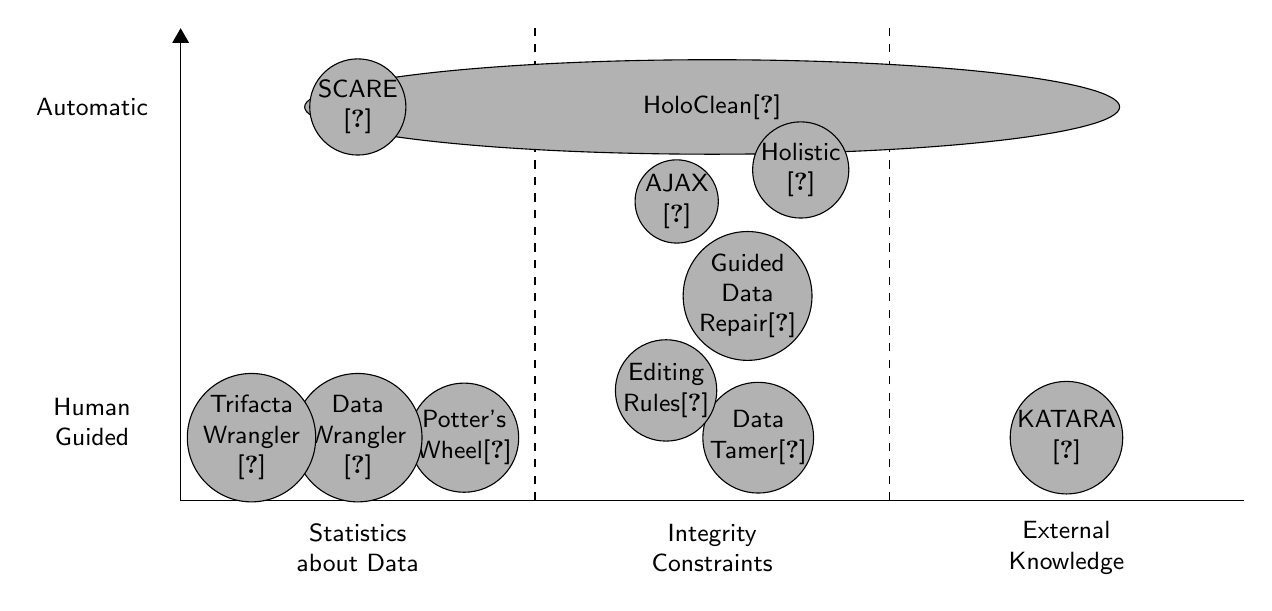
\begin{tikzpicture}[
    xscale=4.5, yscale=4,>=triangle 60,font=\sffamily,
    tool/.style={
      circle,
      draw=black,
      fill=black!30,
      inner sep=0pt,
      minimum size=25pt,
      align=center
    }
  ]
  \small  
  
  \begin{scope}
    \draw[black,] (-1.5,-0.25) -- (1.5,-0.25) ;
    \draw[black,->] (-1.5,-0.25) -- (-1.5,1.25) ;
    \draw[black,dashed] (-0.5,-0.25) -- (-0.5,1.25) ;
    \draw[black,dashed] (0.5,-0.25) -- (0.5,1.25) ;
    
    \draw[tool] (0,1) ellipse (1.15 and 0.15) node {\holoclean{}\cite{holoclean}};
    
    \node[tool] at (1,-0.05) {KATARA\\\cite{katara}};
    
    \node[tool] at (0.13,-0.05) {Data\\Tamer\cite{data_tamer}};
    \node[tool] at (-0.13,0.1) {Editing\\Rules\cite{editing_rules}};
    \node[tool] at (0.1,0.4) {Guided\\Data\\Repair\cite{gdr}};
    \node[tool] at (-0.1,0.7) {AJAX\\\cite{ajax}};
    \node[tool] at (0.25,0.8) {Holistic\\\cite{holoclean}};
    
    \node[tool] at (-0.7,-0.05) {Potter's\\Wheel\cite{potters_wheel}};
    \node[tool] at (-1,-0.05) {Data\\Wrangler\\\cite{data_wrangler}};
    \node[tool] at (-1.3,-0.05) {Trifacta\\Wrangler\\\cite{trifacta_wrangler}};
    
    \node[tool] at (-1,1) {SCARE\\\cite{scare}};
    
    \node[align=center] at (-1.75,1) {Automatic};
    \node[align=center] at (-1.75,0) {Human\\Guided};
    
    \node[align=center] at (1,-0.4) {External\\Knowledge};
    \node[align=center] at (0,-0.4) {Integrity\\Constraints};
    \node[align=center] at (-1,-0.4) {Statistics\\about Data};
  
  \end{scope}
\end{tikzpicture}

\end{document}